\documentclass{book}
\usepackage{fancyhdr}
\pagestyle{fancy}
% with this we ensure that the chapter and section
% headings are in lowercase.
\renewcommand{\chaptermark}[1]{%
        \markboth{#1}{}}
\renewcommand{\sectionmark}[1]{%
        \markright{\thesection\ #1}}
\fancyhf{} % delete current header and footer
\fancyhead[LE,RO]{\bfseries\thepage}
\fancyhead[LO]{\bfseries\rightmark}
\fancyhead[RE]{\bfseries\leftmark}
\renewcommand{\headrulewidth}{0.5pt}
\renewcommand{\footrulewidth}{0pt}
\addtolength{\headheight}{0.5pt} % space for the rule
\fancypagestyle{plain}{%
   \fancyhead{} % get rid of headers on plain pages
   \renewcommand{\headrulewidth}{0pt} % and the line
}




%\documentclass[a4paper,12pt]{book}
%\usepackage[T1]{fontenc}
\usepackage [isolatin]{inputenc} % fontes avec caracteres accentues
\usepackage{graphicx} % inclusion de figures
\usepackage{listings}

\begin{document}

\title{\emph{NPTool 1.0 User Guide}}
\author{Adrien MATTA}

\maketitle 
\pagebreak
\tableofcontents % la table des matieres
\pagebreak

\chapter[NPTool]{NPTool}
\section {Introduction}

NPTool, Nuclear Physics Tool, aim to be a coherent set of programm usefull for Nuclear Physicist, especially those studying structure experimentally. Because each experiment is differents, people get used to exchange code and modified it to their needs. What NPT do is provinding an (try to be) universal framework so user can add their own functionnalities and share it with their collaborators. Geant4 and ROOT are now popular toolkit among the community, that's why NPTool use them widely and try to give a step by step process to use them efficiently.

In NPTool analysis and simulation are linked together. The proposed way of working is to generate an experiment like set of data and then annalysing with the future analysis code. Working this way help saving time by doing the biggest part of the analysis work in advance. It also help to understand what happen during analysis. 

				\begin{figure}[!htbp]
					\centering
					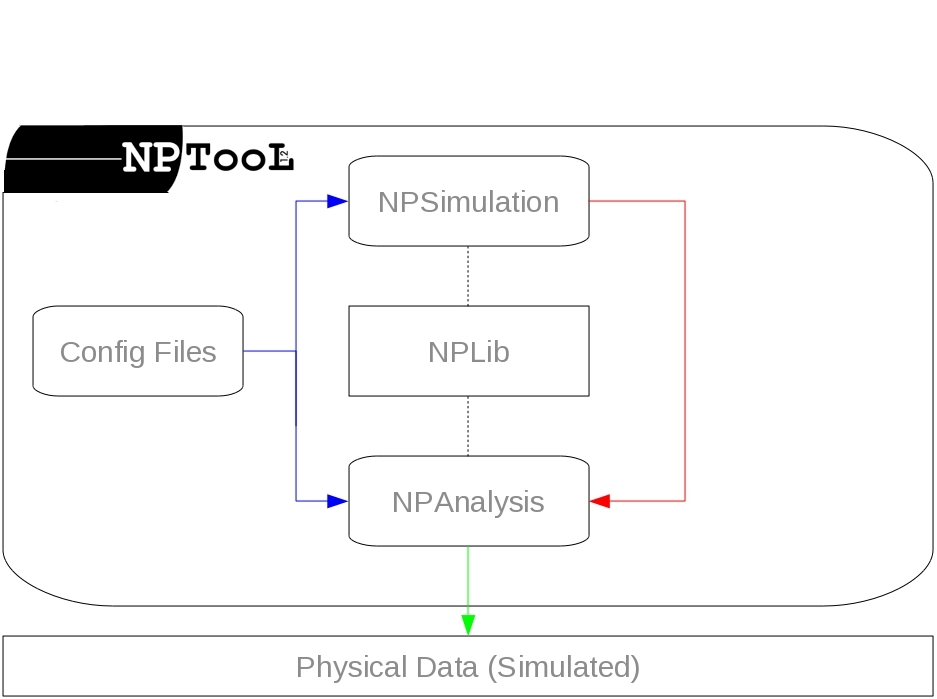
\includegraphics[width=1\textwidth]{./pictures/nptool_scheme_Sim.png}
					\caption{ \emph{Phase 1: Preparing an experiment} }
				\end{figure}

				\begin{figure}[!htbp]
					\centering
					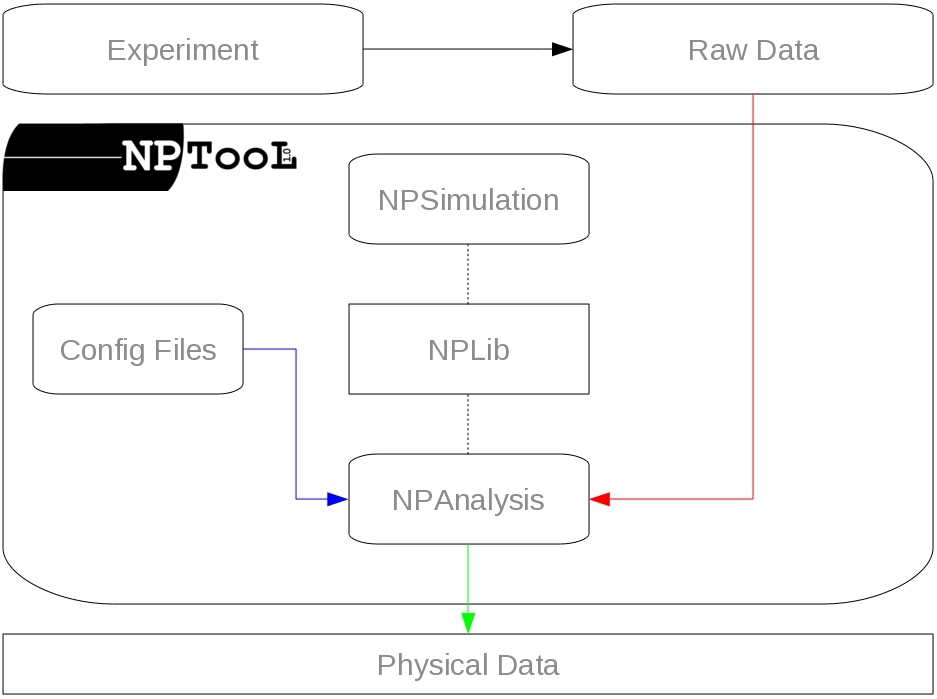
\includegraphics[width=1\textwidth]{./pictures/nptool_scheme_Ana.png}
					\caption{ \emph{Phase 2: Analysing an experiment} }
				\end{figure}
				
\chapter[NPSimulation]{NPSimulation}

\section{NPSimulation}

NPSimulation is build on top of Geant4. It's provide a coherent and modular sets of classes that can be easily modified for your purpose.

\subsection{ The way it's work }

Because NPS is build on top of Geant4, you need C++ knowledge and Geant4 skills to understand how NPS work. NPS is a build as a modular basis that fit Nuclear Physicist needs: 
	\begin{itemize}
		\item Generate Nuclear Physics Event (such as a transfert, a beam, an ion source,... ) 
		\item Mange Detectors geometry (Number of module, positionning...)
	\end{itemize}

NPS used two input files, one for the EventGenerator, and one for the Detectors Geometry. Those file are regroup in the \$NPT/Input directory wher you can find the EventGenerator and the DetectorConfiguration folder. If you want to add a new case you just have to create a new file in those directory. Note that files in the input directory are token readable file. It mean that they are not compile with the code, just read at each programm lauch. This way you can change the position of your detector or the energy of your beam for example without recompile the code. You can also quickly exchange your file with collaborators.

\subsection{ Running a simulation with existing detectors and event generator }

Running a NPSimulation is quite simple, first, start a console terminal (shell) and put your self in the NPS directory. If you have add the environment variable correctly you can use the \emph{NPS} short cut that open the NPSimulation directory.
	
	\begin{footnotesize}
	\begin{center}
	\begin{tabular}{|p{\textwidth}|}
		\hline
			[myName@myDomain$\sim$ ]\${} NPS
			
			[myName@myDomain$\sim$NPSimulation]\${} Simulation myReaction myDetector
		\\
		\hline
	\end{tabular}
	\end{center}
	\end{footnotesize}
	
\emph{NB: order of arguments is essential. Both file need to be in the associated directory (see previous section).}

\emph{Simulation} is their a shortcut (or alias) added in the environment variable. In fact Geant4 generate the binari file in the path \$NPS/bin/YourSystem/ where "YourSystem" depend of you compilator and OS (for example \emph{Linux-g++}). Thats why we use a convinient shortcut.

After typing that command you will have a typical shell output of Geant4
\begin{verbatim}
*************************************************************
Geant4 version Name: geant4-09-01-patch-03 (12-September-2008)
                     Copyright : Geant4 Collaboration
                     Reference : NIM A 506 (2003), 250-303
                           WWW : http://cern.ch/geant4
*************************************************************
\end{verbatim}

Followed by the echo of what are in your input file. Check their that the token are well detected and everything correctly instantiate.

Then you have some standard Geant4 output again and the idle consol where you can tape any of the common Geant4 command, such as launching a run of 100 event:
\begin{verbatim}
Idle> run/beamOn 100
\end{verbatim}

If you want to display the tracking of particle in the differente volume and check the Energy loss you can type the following line. Keep in mind that display slow down the computation.

\begin{verbatim}
Idle> tracking/verbose 1
\end{verbatim}

The simulation will use the configured EventGenerator describe in your input file to generate events. Geant4 will deal with the particle tracking, energy loss, decay,... and the NPS framework generate an output ROOT file in the \$NPT/Output/Simulation directory. Default name for this file is mySimul.root. Since the file is regenerated at each execution, one need to rename it in order to keep it.

\subsection{ Adding a detector to NPS }

First you can have a look to the VDetector.hh file in the \$NPS/include directory. All the detector inherited from this Virtual class (V in VDetector stand for that, following the Geant4 naming convention). A virtual class described what should be the standard features of the inherited object. In this case their is 5 methods: Note thats those method are virtual, wich mean they are not implemented within this virtual class but in the daughter class. That allow to have the same method implemented differently for each detector. The " = 0 " following the class header mean that compilation failed if the daugter class do not have its own method definition (wich can be eventually empty). A Vector of VDetector is manage by the DetectorConstruction file (see DetectorConstruction.hh and .cc) wich call those method automatically.

	\begin{itemize}
		\item[] ReadConfiguration(string): Read the file describing the Detector Configuration, ie: number of detector, position, and other option
		\item[] ConstructDetector(G4LogicalVolume*): Argument is the world volume. The method construct the volume
		\item[] ReadSensitive(const G4Event*): Read the scorer associate the to the sensitive method
	\end{itemize}
	
	
The two last methods are followed by a "{}" wich mean you are free to implemented or not. If not they will remain empty.
	\begin{itemize}
		\item[] InitializeRootOutput(): Instantiate a new Root Data object (see NPLib) and associate it to a new branch
		\item[] InitializeScorers(): Initialize the scorer (see GeneralScorer.hh and Geant4 Documentation)
	\end{itemize}


\end{document}

